\subsection{子領域における地形の取り扱い} \label{subsec:nest_topo}
%------------------------------------------------------
ネスティング実験では、一般的に、親領域と子領域の間で空間解像度が異なるため地形の解像度も異なる。
子領域の緩和領域(第\ref{subsec:buffer}節)では、親領域の大気データにナッジングを行うが、
2つの領域間で地形の表現が異なると、ナッジングに必要な大気データが存在しないことがある。
その場合、外挿などにより大気データを見積もることになるが、見積もりが悪いと不整合が生じる。
%
こういった不整合を無くすため、\scalerm では、ネスティング計算を行う場合、
子領域の緩和領域では親領域の地形をコピーする「地形コピー」機能が推奨されている。
この機能を使えば、図\ref{fig_topocopy}に示すように、子領域の緩和領域は
完全に親領域の地形と一致させることができる。
さらに、地形の解像度を内側にいくに従って徐々に高めていくため、
緩和領域の内側に地形遷移領域を設定し、そこでは親領域と子領域の地形をある割合で重み付けした値を与える。
地形遷移領域の幅は、デフォルト設定では緩和領域と同じ幅である。
さらに内側の内部領域では完全に子領域自身の解像度に応じた地形を与える。
実験セット一式準備ツール(第\ref{sec:basic_makeconf}節) を利用する場合には
地形コピー機能は自動的に適用される設定となっている。


ここで説明する地形コピーの設定を記述した\verb|pp.d0*.conf|ファイルは、サンプル設定ファイル
\verb|${Tutorial_dir}/real/sample/USER.online-nesting.sh|を
USER.shに置き換えて、実験セット準備ツールを実行した場合に作成される。
説明を読み進める上で参考にしてもらいたい。
%
以降、具体的な設定方法と実行手順を説明する。


\begin{figure}[htb]
\begin{center}
  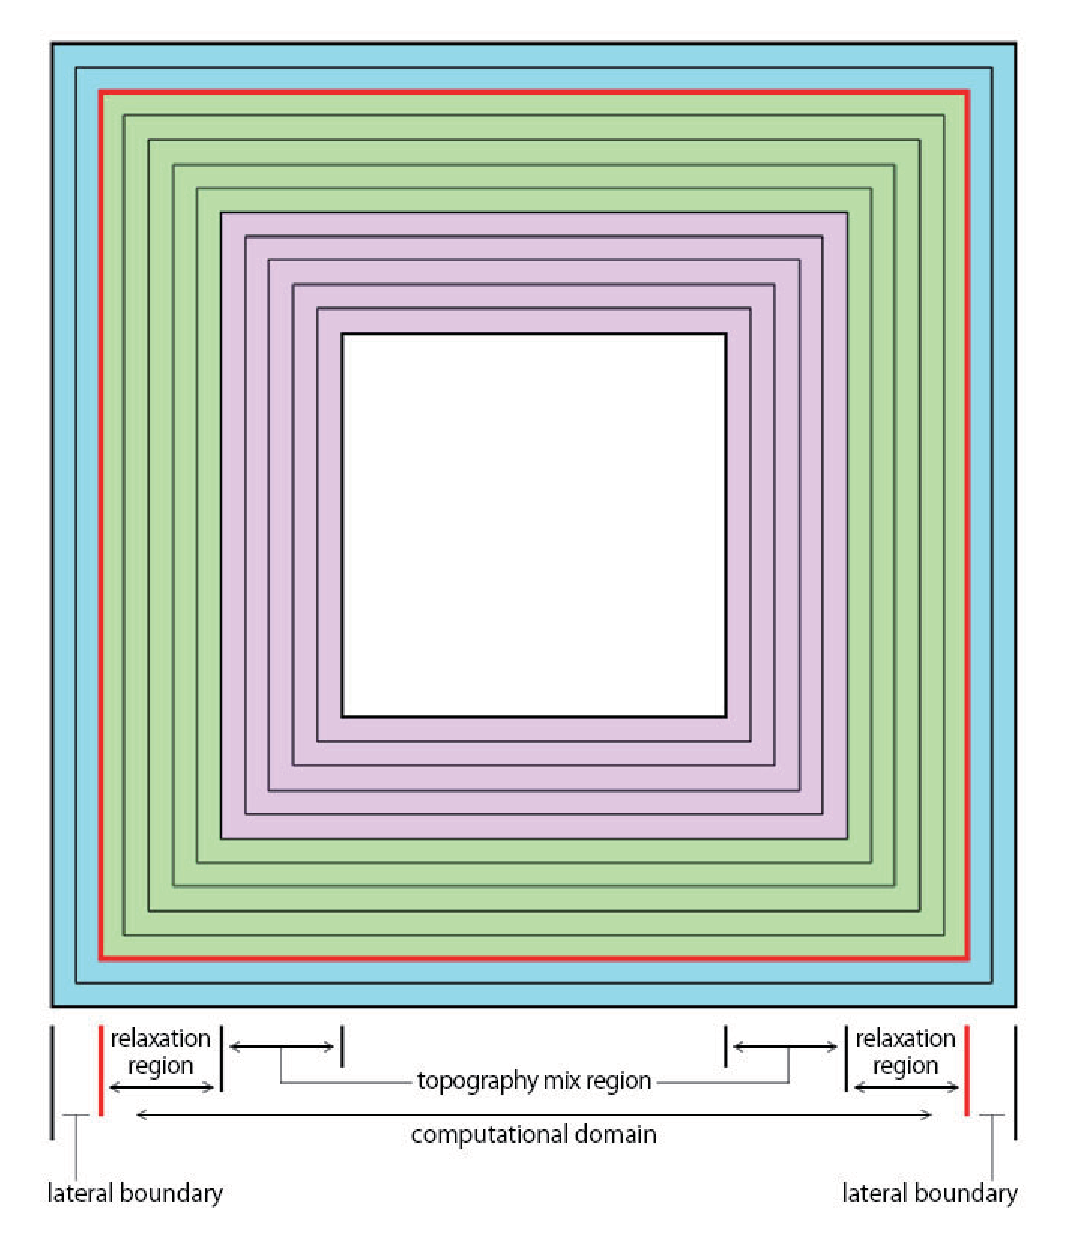
\includegraphics[width=0.4\hsize]{./figure/topo_copy.eps}\\
  \caption{地形コピーを適用した子領域の地形データ水平分布。
最外の水色の格子(\texttt{HALO}領域。格子数は水平差分スキームによって異なる。)は側面境界で、それより内側の赤色の線で
囲われた領域が計算領域である。緑色の部分は緩和領域、桃色の部分は地形遷移領域、
そして最内の白色の部分が子領域の地形をもつ領域である。
地形遷移領域では外側から内側にかけて徐々に親領域の地形データから子領域の地形データへ遷移する。}
  \label{fig_topocopy}
\end{center}
\end{figure}


\subsubsection{地形コピー機能のための設定}

まず親領域の地形データ作成時(\verb|scale-rm_pp|)に
計算領域の大きさを子領域へ伝えるためにカタログファイルを出力するよう設定する。
具体的には、\verb|pp.d01.conf|に下記の設定が必要となる。\\

\noindent {\small {\gt
\ovalbox{
\begin{tabularx}{150mm}{lX}
\verb|&PARAM_DOMAIN_CATALOGUE|  & \\
\verb| DOMAIN_CATALOGUE_FNAME  = "latlon_domain_catalogue.d01.txt",| & カタログファイルのファイル名\\
\verb| DOMAIN_CATALOGUE_OUTPUT = .true.,| & カタログファイルを出力するかどうか \\
\verb|/|  & \\
\end{tabularx}
}}}\\

\noindent その他の設定項目は通常通りで良い。編集ができたら親領域の地形データ作成を実行する。
ここで、出力データは、\verb|topo_d01.pe***.nc|というファイル名で保存されていることを想定する。
次に、子領域の\verb|pp.d02.conf|ファイルを編集する。\\

\noindent {\small {\gt
\ovalbox{
\begin{tabularx}{150mm}{lX}
\verb|&PARAM_NEST| & \\
\verb| USE_NESTING               = .true.,| & \\
\verb| OFFLINE                   = .true.,| & \\
\verb| OFFLINE_PARENT_PRC_NUM_X  = 2,     | & 親領域の\verb|PRC_NUM_X| \\
\verb| OFFLINE_PARENT_PRC_NUM_Y  = 2,     | & 親領域の\verb|PRC_NUM_Y| \\
\verb| OFFLINE_PARENT_KMAX       = 36,    | & 親領域の\verb|KMAX|      \\
\verb| OFFLINE_PARENT_IMAX       = 45,    | & 親領域の\verb|IMAX|      \\
\verb| OFFLINE_PARENT_JMAX       = 45,    | & 親領域の\verb|JMAX|      \\
\verb| OFFLINE_PARENT_LKMAX      = 5,     | & 親領域の\verb|LKMAX|     \\
\verb| LATLON_CATALOGUE_FNAME    = "latlon_domain_catalogue.d01.txt",| & 親領域のカタログファイル  \\
\verb|/| &\\
 & \\
\verb|&PARAM_CNVTOPO|  &\\
\verb|     〜 中略 〜| & \\
\verb| CNVTOPO_copy_parent     = .true.,| & 地形コピー機能を適用するかどうか\\
\verb|/| &\\
 & \\
\verb|&PARAM_COPYTOPO| & \\
\verb| COPYTOPO_IN_BASENAME   = "topo_d01",| & 親領域の地形データの頭 \\
\verb| COPYTOPO_ENTIRE_REGION = .false.,|    & 子領域の全域に親領域の地形をコピーするかどうか\\
\verb| COPYTOPO_LINEAR_H      = .true.,|     & \\
\verb|/| & \\
\end{tabularx}
}}}\\

\noindent 
地形コピーを用いるには、\namelist{PARAM_CNVTOPO}の\nmitem{CNVTOPO_copy_parent}に\verb|.true.|を設定する。
\nmitem{COPYTOPO_ENTIRE_REGION}は、全領域でコピーするかどうかを決定するオプションである。
このスイッチを\verb|.true.|にすると、図\ref{fig_topocopy}に示されたすべての領域で親領域の地形が完全にコピーされる。
3つ目の\nmitem{COPYTOPO_LINEAR_H}は地形遷移領域の遷移具合を調整するスイッチである。
\nmitem{COPYTOPO_LINEAR_H}が\verb|.true.|だと、親領域の地形と子領域の地形の混合割合が
線形的に変化するのに対し、\verb|.false.|だと指数関数的に変化する。
緩和領域の設定と同じ要領で、\nmitem{COPYTOPO_TRANSITION_DX}、\\
\nmitem{COPYTOPO_TRANSITION_DY}、
及び、\nmitem{COPYTOPO_TRANSFACT}により任意の幅に設定することができる。


地形コピー機能では、オフライン・ネスティング実験の
フレームワークを利用するため、\namelist{PARAM_NEST}の全ての項目を追記する必要がある。
設定変数の詳しい説明は、\ref{subsec:nest_offline}節の
オフライン・ネスティング実験の説明を参照してほしい。


\subsubsection{地形の作成}

地形コピー機能を使用する場合(つまり、ネスティング計算の場合)、
子領域は親領域の地形データ作成時に出力されるカタログデータを必要とするため、
地形データの作成は、親領域から順番に実行する。
3つ以上の領域がある場合も、手続きは同様である。
下記の例で、\verb|[PRCnum]|はそれぞれの計算で必要なMPIプロセス数を示す。

\begin{verbatim}
 $ mpirun -n [PRCnum] ./scale-rm_pp pp.d01.conf
 $ mpirun -n [PRCnum] ./scale-rm_pp pp.d02.conf
 $ mpirun -n [PRCnum] ./scale-rm_pp pp.d03.conf
\end{verbatim}

